\capitulo{2}{Introducción}
% Se pueden añadir todas las subsecciones que queramos o necesitemos.

(Descripción del contenido del trabajo y de la estructura de la memoria y del resto de materiales entregados.)

Este trabajo surge de una visita a la asociación de Parkinson Burgos, los fisioterapeutas deseaban alguna solución para no estar pendientes continuamente de que las personas andaran correctamente erguidos. 

Por otro lado, hoy en día estamos mucha parte de nuestro tiempo sentados, no siempre adoptando una buena postura.

Este problema no es único de personas con alguna afectación, sino que todos en algún momento adoptamos una mala postura y en algunos casos de forma continuada por lo que puede afectarnos a largo tiempo si no adoptamos medidas para corregir esa postura. Una mala postura puede producir un deterioro de los músculos, daños musculares, cambios en la morfología de la columna y dificultad para realizar tareas o movimientos.


\section{Conceptos teóricos básicos.} %Explicación de los conceptos teóricos básicos necesarios para que cualquier miembro del tribunal pueda entender el trabajo realizado.
Para llevar a cabo este trabajo hay que comprender su base, en este caso el control postural, qué es, su importancia y todo lo que ello conlleva.\cite{Libro1,Libro2} % Citar el libro

% Referenciar:


Algunos de los conceptos básicos que se deben comprender y que están relacionados o engloban el control postural son:
%Antes de comenzar se deben conocer los siguientes conceptos básicos y componentes que engloban el control postural:

\begin{itemize}
    \item \textbf{Base de sustentación} será la superficie disponible sobre la que al cuerpo apoya su peso. \ref{fig:persona}\footnote{Esta imagen ha sido generada parcialmente empleando la inteligencia artificial DALL·E}
    % Referencias
    % https://www.fisioterapia-online.com/glosario/base-de-sustentacion
    \item \textbf{Área de apoyo} es el área sobre la que el cuerpo descarga su peso de forma efectiva. En el caso de una persona de pie, el área de apoyo será el área correspondiente con la planta de los pies.
    \item \textbf{Centro de masas} \cite{CDM} o CDM es la posición media de todos los centros de masas de las distintas partes del cuerpo. El CDM se encuentra relacionado con el equilibrio. El CDM es el punto de actuación de fuerzas uniformes sobre el objeto. \ref{fig:persona}
    % Referencia:
    %https://es.khanacademy.org/science/physics/linear-momentum/center-of-mass/a/what-is-center-of-mass
    \item \textbf{Centro de presiones} o CDP es la proyección del centro de masas del cuerpo sobre la base de sustentación .\ref{fig:persona}
    \item \textbf{Centro de gravedad} o CDG es el punto del cuerpo donde se ejerce la fuerza de gravedad que afecta a la masa del cuerpo. Existen dos métodos para encontrar el centro de gravedad, el método de balanceo y el método de los pesos. \ref{fig:persona}% Referencia de apuntes de diseño mecánico.

\begin{figure}[h!]
    \centering
    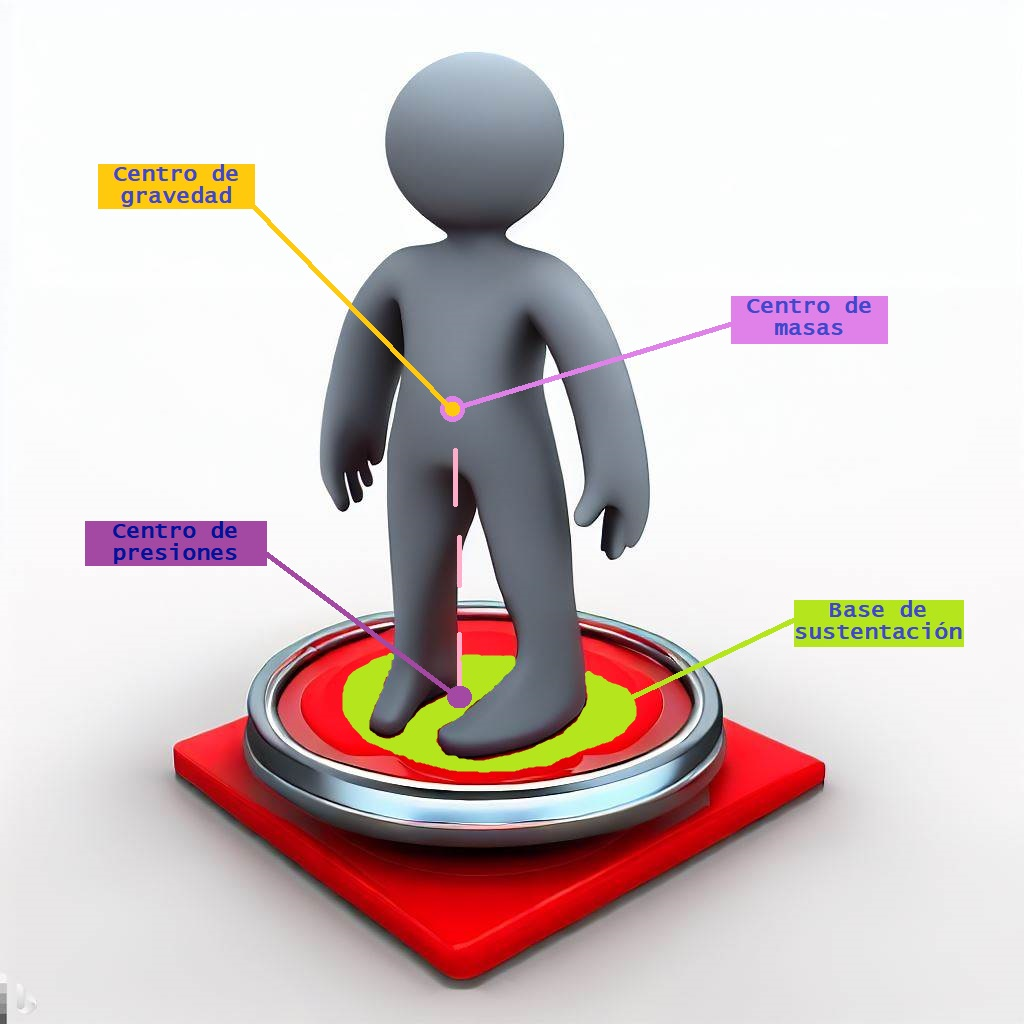
\includegraphics[width=0.5\textwidth]{img/IA_Persona.jpeg}
    \caption{Diagrama de la localización de la base de sustentación y los centros de masas, presiones y gravedad de una persona de pie.}
    \label{fig:persona} % Esta etiqueta es la que permite que se encuentr referenciada en el texto (es muy importante que siempre estén referenciadas en el texto)
\end{figure}
    
    \item \textbf{Postura} es la orientación y alineamiento del cuerpo respecto a su entorno.
    \item \textbf{Orientación postural} es la capacidad de mantener la relación entre las distintas partes del cuerpo y el entorno al realizar una actividad.
    \item \textbf{Sinergia postural} es la relación entre la contracción muscular y las rotaciones articulares para estabilizar la postura.
    \item \textbf{Balanceo postural} es el desplazamiento constante y la corrección del centro de gravedad para mantener la postura.
    \item \textbf{Límite de estabilidad} es el trayecto por el cual una persona puede realizar un movimiento sin perder su equilibrio y también puede realizar ajustes posturales. No se trata de un límite fijo, varía con el tiempo, la tarea que se esté realizando o el entorno en el que se encuentra.
\end{itemize}

La postura nace de la relación entre el entorno, el individuo y la actividad que debe realizar. Y, por tanto, el \textbf{control postural} se define como el control de la posición corporal en el espacio con el fin de obtener la estabilidad y la orientación que necesitamos para poder realizar las actividades diarias, profesión o aficiones. 

La \textbf{estabilidad} es la capacidad de mantener la proyección del centro de gravedad dentro de una base de sustentación, mientras que la \textbf{orientación} es la capacidad de mantener la relación adecuada entre las distintas partes del cuerpo al realizar una tarea teniendo en cuenta el entorno.

Para poder cumplir con el objetivo del control postural el cuerpo tiene que poder anticiparse, mantenerse y reaccionar. Además, el control postural requiere que interaccionen distintos sistemas del cuerpo para abarcar la estabilidad, la percepción de la orientación espacial, el alineamiento del cuerpo, la lucha contra la gravedad al realizar un movimiento y la respuesta a posibles perturbaciones, ya sean de origen sensorial o mecánico.

Principalmente, en el control postural interviene el sistema nervioso, como centro de control, manteniendo la postura y el equilibrio gracias a la recogida e interpretación de información de los receptores y a la producción de órdenes; y, el sistema musculoesquelético, ya que se requiere de una musculatura capaz de adaptarse a los cambios. Además, como seres inteligentes que somos,se utilizan experiencias previas para elaborar el esquema corporal.

Por todo ello se va a conocer más a fondo la relación del sistema nervioso y la postura, algunas estrategias del control postural y su importancia o desarrollo.

%Subseccion
\subsection{El sistema nervioso y la postura.} 
El sistema nervioso se compone de diferentes estructuras como son las neuronas o las células de neuroglia, que se encargan de mantener la homeostasis corporal regulando y coordinando las distintas funciones del organismo.

Asimismo, el sistema nervioso se puede dividir en sistema nervioso central que se encuentra compuesto por la médula espinal y el encéfalo, y el sistema nervioso periférico que está compuesto por ganglios y nervios.
% añadir imagen de los sistemas central y periférico.

El sistema nervioso también se puede dividir en función del tipo de respuestas de las que se encargan, si se encarga de las respuestas involuntarios se trata del sistema nervioso autónomo que, a su vez, se divide en los sistemas simpático y parasimpático. Mientras que, si se encarga de las respuestas voluntarias del organismo se llama sistema nervioso somático.

Los receptores son los que se encargan de recoger la información que se envía al sistema nervioso mediante mecanismos de retroalimentación. Existen numerosos receptores y estos elementos se pueden encontrar en los músculos, para poder detectar el movimiento. Por otra parte, se necesita también la información recogida por la vista, el sistema vestibular del oído interno o las señales procedentes de las modificaciones de presión.

Si en algún caso se producen perturbaciones los receptores detectarán esos imprevistos y proporcionarán información acerca de las nuevas condiciones para así adaptar el tono postural. Por ejemplo, si los receptores de presión de los pies registran el desplazamiento mínimo durante la bipedestación se transmite la información por el nervio periférico, seguido de la medula espinal, el tracto espinocerebeloso y desde el cerebelo a la formación reticular y a los núcleos vestibulares. Si se desplaza la cabeza se crea una aceleración en dirección anterior que se registra y se transmite a los núcleos vestibulares. 

Las reacciones de equilibrio son la respuesta al control postural, los núcleos vestibulares activan la musculatura de la 'core-stability' que está formada por los músculos del suelo pélvico, los músculos profundos paravertebrales y sacrolumbares, y, la musculatura abdominal y lateral. En función del tipo de desplazamiento se activarán una cadena u otra, ya sean la cadena anterior, la posterior, la lateral o combinaciones de las mismas.

\subsection{Estrategias de control postural.} 
El control postural y los ajustes se dan en tronco, tobillos y caderas, de esta forma se puede mantener el equilibrio, creando la estabilidad que posibilita los movimientos al realizar distintas actividades.

Existe un modelo que define 3 elementos que modifican, construyen y mantienen la postura, el \textbf{modelo de sistemas dinámicos de Bernstein}. Los elementos en cuestión son los factores individuales, la tarea a realizar y el entorno. 

Los factores individuales son aquellos pertenecientes a cada individuo, pueden variar su influencia con entrenamiento. Dentro de los factores individuales encontramos los elementos sensitivos que proporcionan información respecto al movimiento y la posición del centro de gravedad. Los elementos sensitivos incluyen las aferencias visuales (posición respecto al entorno), el sistema somatosensitivo (son los receptores de los músculos, la piel u otros tejidos, dan información acerca de las variaciones de la orientación postural) y el vestibular (es básicamente el oído, posición de la cabeza). También encontramos los elementos motores que hacen referencia a las exigencias musculoesqueléticas (fuerza, flexibilidad o alineación de las partes del cuerpo) y neuromusculares (patrones de movimiento y contracción de los músculos)  necesarias para el ajuste postural; y, los elementos cognitivos que refieren a las necesidades psicológicas y cognitivas relacionadas con la actitud postural.

Igualmente, existen diferentes estrategias de control de la postura, como aquellas que se centran en el equilibrio, controlando las oscilaciones o balanceos espontáneos. Algunas de estas estrategias son las de controlar la correcta alineación corporal, minimizando las fuerzas gravitatorias; el suficiente tono muscular mediante el control de la resistencia de un músculo a ser estirado; el correcto tono postural, a partir del control de la fuerza de gravedad; o, el control de las reacciones posturales o de balance mediante ajustes compuestos de reacciones de equilibrio, enderezamiento y de apoyo. 

Por otro lado, la memoria implícita que se da en el cerebelo y en los núcleos basales proporciona información sobre dónde, cuánto y cómo se debe ajustar el tono postural para compensar los desplazamientos.

Otras estrategias para mantener el control postural son las que describen Shumway-Cook y Woollacott, la ‘ankle strategy’ que se basa en la bipedestación mantenida por la base de sustentación pequeña que serán los tobillos, la ‘hip strategy’ que se basa en controlar los centros de masas en un desplazamiento de peso mayor y la ‘stepping strateging’ que se basa en una base de sustentación aún mayor.

\subsection{Desarrollo del control postural.} 
Las necesidades de estabilidad cambian con la tarea que se debe realizar. El desarrollo de control postural en niños se produce en tres etapas, primero, se debe desarrollar el control encefálico, después la sedestación (capacidad de sentarse) y, por último, la bipedestación.

Además, la postura y el equilibrio varían con la edad, por una parte, los niños pequeños\cite{Libro3_pediatria} no tienen suficientemente desarrollado las aferencias sensoriales, y por otra los adultos mayores\cite{Libro4_mayores} presentan involución cognitiva de sus estructuras cerebrales, todos ellos ven disminuido el control postural.

Asimismo, pacientes con traumatismos craneoencefálico, esclerosis múltiple, infartos u otras lesiones en el sistema nervioso central pueden tener afectado alguno de elementos implicados en el control de la postura y por lo que su control postural se verá afectado. En algunos casos también influyen los factores psicológicos, una persona con depresión o un problema de atención también puede llegar a influir sobre ese control postural.

\begin{comment}
    
%Sub-subseccion
\subsubsection{Sub Subsección}

\subsubsection{Sub Subsección}

En esta sección y el resto de secciones de la memoria puede ser necesario incluir listas de items.

% Listas de puntos 
\begin{itemize}
    \item item1
    \item item2
    \item item3
\end{itemize}

Listas enumeradas.
% Enumeraciones
\begin{enumerate}
    \item item1
    \item item2
    \item item3
\end{enumerate}

Figuras, como la figura \ref{fig:escudo} que aparece en la página \pageref{fig:escudo}. 

Puedes aprender más de las figuras en la dirección \url{https://es.overleaf.com/learn/latex/Inserting_Images} % más informacion de como utilizar figuras

% Inicio de la figura
\begin{figure}[h]
    \centering
    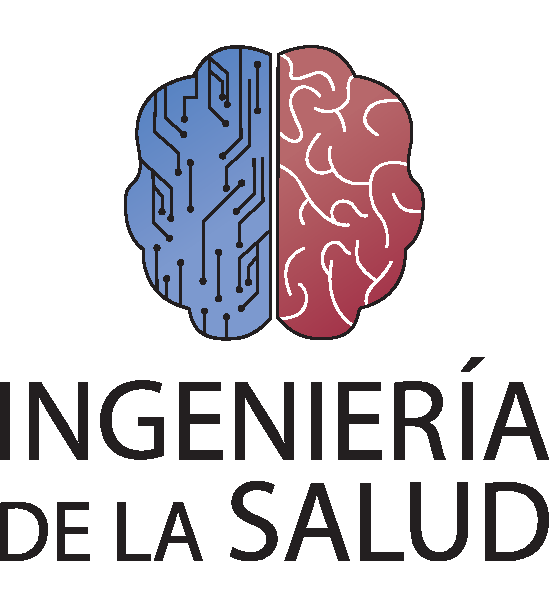
\includegraphics[width=0.25\textwidth]{img/escudoSalud.pdf}
    \caption{Pie de la figura}
    \label{fig:escudo} % Esta etiqueta es la que permite que se encuentr referenciada en el texto (es muy importante que siempre estén referenciadas en el texto)
\end{figure}


También se pueden insertar tablas como \ref{tab:my-table}, que ha sido generada con \url{https://www.tablesgenerator.com/}. % Este enlace permite crear tablas y te genera el código latex

% Ejemplos de tablas
\begin{table}[]
\begin{tabular}{lll}
a & b & c \\
1 & 2 & 3 \\
4 & 5 & 6
\end{tabular}
\caption{}
\label{tab:my-table}
\end{table}

Es necesario que todas las figuras y tablas aparezca referenciadas en el texto, como estos ejemplos.

Todos los conceptos teóricos deben de estar correctamente referenciados en la bibliografía. Por ejemplo, aquí estoy citando la página de \LaTeX{} de Wikipedia \cite{wiki:latex}. %El comando \cite permite referenciar las citas bibliográficas, siempre se tienen que referenciar las citas de la bibliografía.
\end{comment}

También puede ser necesario utilizar notas al pie \footnote{como por ejemplo esta}, para aclarar algunos conceptos.


\section{Estado del arte y trabajos relacionados.}

\begin{comment}
Revisión bibliografica de que se está haciendo en la industria o la academia relativo al problema que se está tratando.

Enumeración y resumen de todos los trabajos relacionados de interés.


También se puede incluir que existen gran variedad de dispositivos cuyo fin es el de medir o controlar la postura.
\end{comment}
En la actualidad existen multitud de dispositivos electrónicos \cite{dispositivos} compuestos de distintos sensores, actuadores y algoritmos cuya finalidad es algún tipo de control postural, ya sea regulándola o modificando la postura. Se podrían diferenciar según su aplicación final: 
\begin{itemize}
    \item Mejora de la estabilidad del equilibrio de las personas con alguna alteración en el control postural como pueden ser personas con parálisis cerebral, esclerosis múltiple, Párkinson… 

    \item Prevención de una mala postura en personas que están sentadas o realizando alguna actividad. 

    \item Monitorización de la postura como feedback para mejora de ergonomía en diferentes personas, por ejemplo, en atletas\cite{Deportistas_1,Deportistas_2}. 
\end{itemize}

Es necesario conocer las especificaciones que requerirán los dispositivos en función de la aplicación a la que se encuentren destinados. Algunas especificaciones que se deben tener en cuenta al diseñar o elegir un dispositivo electrónico de control postural son: 
\begin{itemize}
    \item Precisión y fiabilidad de los sensores y actuadores para detectar y responder correctamente a los cambios en la postura. 

    \item Facilidad de uso y comodidad, para que se adapte a las necesidades del usuario y a su actividad. 

    \item Autonomía y conectividad del dispositivo para que se adapte a las actividades que realiza el usuario. 
\end{itemize}

Por todo ello se realiza un estudio de distintos dispositivos que existen en la actualidad cuya finalidad u funcionamiento es similar al objetivo de este proyecto. 

\subsection{Dispositivos de control postural} 
\begin{itemize}
    \item En el grupo de investigación de Redes de Neuronas Artificiales y Sistemas Adaptativos de la \textbf{Universidad de A Coruña} junto con la empresa Bioback de Puerto Rico se ha desarrollado un dispositivo inteligente no invasivo para la corrección postural utilizando estimulación vibratoria\cite{dispositivoUAC}. Este dispositivo se basa en el uso de ‘Biofeedback’ como medio de aprendizaje, condicionando las rutinas de los individuos.  \newline El dispositivo está compuesto por una parte de hardware que incluye 3 secciones que se colocan en 3 partes de la columna vertebral (zona cervical (C1-T1), zona torácica (T1-L1) y zona lumbar (L1-L5)) siguiendo el modelo Goodvin. Cada sección del hardware esta formada por un grupo de sensores IMU (Unidad Inercial de Medida) que están compuestos por un acelerómetro triaxial, un giroscopio triaxial y un magnetómetro triaxial, que permiten obtener una lectura completa de la inclinación, la torsión y la flexión. Los IMUs son capaces de medir de 0º a 360º en cada eje, con una resolución de 0,1. Además, el dispositivo electrónico incluye un Sistema experto que incluye un módulo de conexión Bluetooth, una tarjeta SD para guardar los datos, una batería de litio interna recargable (16 horas de autonomía) y el sistema de vibración.  \newline Los datos son procesados por un software que permite conocer en cualquier momento la posición exacta y puede reproducir el movimiento de cada sección de la columna vertebral. Por otro lado, gracias al software se puede configurar el umbral de desviación, las secciones activadas y el tiempo de activación para proporcionar la señal de retroalimentación, es decir, el estímulo vibratorio. 

    % Referencia:
    % Rabuñal, J. R., Cuevas, J., Nogueira, M., Rodríguez-Sotillo, A., Patiño, S., Rivas, A., & Pazos, A. (2015). Dispositivo Inteligente para el Aprendizaje de la Correción Postural mediante Estimulación Vibratoria. Especial Innovación, 6. Retrieved from: http://seis.es/wp-content/uploads/2018/02/Revista-109.pdf#page=6  

    \item \textbf{Wireless wearable T-shirt}\cite{wirelessT-shirt}: es prototipo de una camiseta inteligente permite controlar la postura ya que incluye un sensor inductivo adherido a la camiseta de licra además de un sistema de biofeedback constante gracias a la conexión con aplicación y la señal de vibración que indica una mala postura. El sensor inductivo está formado por un alambre de cobre de un milímetro de diámetro que recorre toda la camiseta en zigzag y cuyo alargamiento modifica el valor de la impedancia generando un voltaje que se puede medir, y por lo tanto, al enderezar o encoger el cuerpo se puede observar un cambio de voltaje que se puede medir y que permite diferenciar entre una buena postura o una mala postura. Dispone de un circuito complementario al que se acopla el sensor y que incluye el módulo bluetooth, el módulo con el motor de vibración, el microprocesador y la batería. En el caso de que el algoritmo detecte una mala postura, se genera la señal vibratoria para incentivar al usuario a modificar su postura. Se ha comprobado la utilidad del dispositivo comparando las respuestas con otros métodos ópticos obteniendo resultados satisfactorios. Este proyecto es solamente un prototipo y no tiene sistema de calibrado y no tiene en cuenta que cada persona no tiene las mismas características físicas por lo que no es posible utilizar el mismo dispositivo para todas las personas. Por otro lado, al ser un prototipo no se han realizado las suficientes pruebas sobre cómo afectaría el sensor en contacto con la piel durante un tiempo de uso continuado.
    % Referencias:
    % E. Sardini, M. Serpelloni and V. Pasqui, "Wireless Wearable T-Shirt for Posture Monitoring During Rehabilitation Exercises," in IEEE Transactions on Instrumentation and Measurement, vol. 64, no. 2, pp. 439-448, Feb. 2015, doi: 10.1109/TIM.2014.2343411. Retrieved from: https://ieeexplore.ieee.org/document/6879298

    \item \textbf{Sistema Upright Go 2}\cite{UprightGo1,UprightGo2,UprightGo3,UprightGo4,UprightGo5,UprightGo6}: es un dispositivo que se adhiere entre los omoplatos de la persona y controla la postura, enviando una vibración cuando se detecta una mala postura, para que el usuario modifique su postura. Está principalmente diseñado para personas que se encuentran sentadas frente a una pantalla. Se basa en el uso de 2 sensores de movimiento, giroscopios. Mide la postura 100 veces en un segundo.
    % Referencias:
    % https://store.uprightpose.com/products/upright-go2  
    % https://www.amazon.es/UpRight-Dispositivo-corrector-postura-corporal/dp/B0747YHYZF?th=1  
    % https://mejorconsalud.as.com/upright-dispositivo-mejorar-postura/  
    % https://www.uprightpose.com/en-de/science/ 

    % Manuales: https://manuals.plus/m/68128076f22ff3a39835113b4c030ef7df2065f3f8a573f0c54db8de4d0e5ad8_optim.pdf  o  https://www.manualslib.com/manual/1312878/Upright-Go.html?page=21#manual  
    
    
    \item \textbf{Hipee Smart Posture Correction}\cite{Hipee1,Hipee2}: es un dispositivo similar al sistema Upriht Go creado por la empresa Xiami. Es un dispositivo que se ajusta a la parte superior de la espalda del usuario a modo de collar y que en base a un sistema de sensores indica la postura del usuario. En caso de una mala postura, al superar el ángulo (ángulos entre 5 y 20º) que se ha incluido en la aplicación durante un tiempo determinado, se emite una señal de vibración a modo de recordatorio para que la persona recupere la postura correcta. Se puede conectar con su aplicación de monitorización vía Bluetooth, pudiendo obtener un informe diario y conocer los registros de los últimos 30 días. Tiene un peso de unos 50 gramos, una autonomía de hasta 90 horas y un precio aproximado de 30€. Está principalmente diseñado para un uso mientras la persona se encuentra sentada o de pie sin moverse mucho. 
    % Referencias: 
    % https://xiaomipedia.com/p/hipee-posture-correction-device/    
    % https://www.lasexta.com/tecnologia-tecnoxplora/gadgets/este-collar-inteligente-que-vende-xiaomi-evita-malas-posturas-espalda_202010225f91862051dc2300012741ef.html 

    \item \textbf{Sistema SPINE 3D}\cite{SPINE3D}: es un sistema de evaluación de patologías vertebrales y alteraciones posturales usando la detección optoelectrónica tridimensional, con unas cámaras RGB infrarrojas (Cámaras ToF) que identifican de forma automática los puntos de referencia en la espalda del paciente y además permiten su modificación de forma manual. Se obtiene una adquisición 3D de la parte superior del cuerpo teniendo en cuenta la longitud, la inclinación y el desequilibrio, desviación y rotación de la columna en los planos coronal, sagital y transversal, lo que ofrece al profesional un estudio completo del paciente y que le permitirá mejorar su diagnóstico y tratamiento. Se trata de un dispositivo que se utiliza de forma estática, donde el paciente se encuentra de pie y con la espalda descubierta delante del aparato. 
    % Referencias:
    % https://www.sensormedica.com/es/spine3d/   

    \item \textbf{Sistema dinámico de medición de la presión del pie}\cite{SisDinPresionPie}: se trata de un manómetro médico, que obtiene la información basándose en el análisis de la marcha y el análisis de la presión que se ejerce sobre los pies y su distribución por la planta del pie. Para obtener la información sigue 3 pasos, primero, divide el monitor de presión del pie en 4 partes iguales donde la presión debe estar distribuida aproximadamente a un 25\% por cada parte, seguidamente, realiza 18 fotogramas por segundo del estado de la presión del pie y se comprueba que la distribución de la presión de cada pie se encuentre aproximadamente en un 30\% para la zona del talón y un 20\% para la zona delantera, por último, compara los resultados promedios de los fotogramas. Se puede usar de forma estática o de forma de dinámica para medir la postura. 
    % Referencias:
    % https://alfoots.com:5000/sub/02_sub/02_sub02.php   

    \item \textbf{Sistema 3D BAK}\cite{3DBAK}: es un sistema de adquisición de la morfología del paciente que utiliza cámaras de alta resolución autocalibrables en diferentes planos para realizar reconstrucciones en 3D. Además, se miden las simetrías estructurales, la rotación de las articulaciones y la desviación de la columna vertebral y se evalúan en base a la Biomechanical Postural Index Scale. Se devuelve un informe imprimible con la información de la rotación individual de cada vertebra y las extremidades y el alineamiento y desviaciones de la columna en 24 indicadores BPI y sus valores, para simplificar la tarea de diagnóstico del profesional. Es un dispositivo no invasivo y el 95,8\% de los resultados son exactamente iguales a los que se obtendrían al usar rayos X. 
    % Referencias:
    % http://diasu.com/sistemi-biometrici/  

    \item \textbf{Sistema PGO}\cite{SisPGO}: es un sistema de medición de la marcha que analiza varios parámetros que afectan a la marcha, mediante el uso de cámaras colocadas en distintos ángulos, un potente software y una cinta de correr. Analiza la inclinación de la cabeza, el nivel de la postura de cabeza hacia delante, el nivel de cifosis, la diferencia de amplitud del movimiento de entre los brazos, la diferencia de altura de los lados de los hombros y de la pelvis, la diferencia entre la longitud de los pasos, la pronación y supinación y la marcha del dedo del pie. 
    % Referencias:
    % https://alfoots.com:5000/sub/02_sub/02_sub02.php   

    \item \textbf{Sistema GPA}\cite{SisGPA}: Es un sistema de medición corporal a partir de la presión que se ejerce en la planta del pie y el análisis de la marcha. El dispositivo utiliza distintas cámaras para analizar las vistas anterior, superior y lateral, además también incluye una placa con una serie de sensores de presión. Este dispositivo permite realizar una evaluación estática, una evaluación dinámica y una podoscopia.  
    % Referencias:
    % https://alfoots.com:5000/sub/02_sub/02_sub02.php 
\end{itemize}

\subsection{Sistemas no específicos de control postural que podrían ser empleados para el control postural} 
\begin{itemize}
    \item \textbf{Sistema PLIANCE}\cite{Pliance1,Pliance2}: es un sistema inalámbrico de medición de la presión. Utiliza una matriz de transductores capacitivos Novel para medir la distribución de la carga sobre cualquier superficie. Los elementos y las características del transductor son fabricados por la propia empresa (Novel) de forma personalizada en función de las necesidades de medición. Este dispositivo se puede comunicar con el PC utilizando USB, Bluetooth y también admite almacenamiento de los datos en una tarjeta SD. Se ha añadido este sistema porque en base a la distribución de la presión en los pies se puede determinar la postura. 
    % Referencias:
    % https://www.novelusa.com/products 
    
    \item \textbf{Siren Diabetic Socks}\cite{SirenSocks1,SirenSocks2}: son unos calcetines inteligentes diseñados para la prevención de úlceras en los pies de personas diabéticas. Este sistema incluye unos sensores de temperatura que recogen las medidas de temperaturas cada 10 segundos con una capacidad para medir entre 20ºC y 40ºC. Los datos recogidos por los sensores se envían a un equipo especializado de profesionales sanitarios que procesan esos datos. Estos calcetines están incluidos en distintos seguros de salud como es Medicare. Estos calcetines previenen de posibles úlceras, gangrena y una posterior posible amputación. Estos calcetines monitorizan la temperatura de la parte inferior de los pies. Estos calcetines deben ser prescritos por un profesional. Consta de una aplicación móvil que emite alertas ante aumentos significativos de temperatura. De este dispositivo se podría utilizar el formato de calcetines, utilizando sensores de presión o similar en vez de sensores de temperatura, o de forma complementaria.

    % Referencias:
    % https://www.siren.care/for-patients
    % 

    \item \textbf{Dispositivos inteligentes en la práctica de yoga}\cite{YOGA}: existen distintos dispositivos inteligentes enfocados a la mejora de la práctica de yoga que monitorizan las posturas que adopta la persona durante la realización de este deporte. Por ejemplo existen unos leggins inteligentes que incluyen sensores y un dispositivo de feedback vibratorio, Nadi X, Smart Yoga Pants\cite{NadiX}, creado por la empresa Wearable X. Otro de los dispositivos es una esterilla de yoga con sensores de presión para el control de las posturas de este deporte. 

    
\end{itemize}

En base a los dispositivos vistos se pretenderá realizar un prototipo de uso general basándose en sensores capaces de registrar la inclinación de una persona, es decir detectar una buena o mala postura. El dispositivo será inalámbrico y vendrá acompañado por una aplicación móvil que proporcionará una mejor experiencia de usuario y un mayor conocimiento de la postura del usuario. Además, el dispositivo al ser inalámbrico deberá contar con una batería de alimentacion y deberá tener la menor cantidad de cables posible para la mayor comodidad del usuario.
